\documentclass{article}
\usepackage[utf8]{inputenc}
\usepackage{graphicx}
\graphicspath{ {./images/} }
\usepackage{amsmath}
\usepackage{hyperref}
%\usepackage[english]{babel}

\usepackage[left=2cm,right=1cm, top=2cm,bottom=2cm,bindingoffset=0cm]{geometry}

\renewcommand{\normalsize}{\fontsize{14}{18pt}\selectfont}

\title{ Analyzis of E.coli strains for outbreak investigation via identification pathogenic genes    }
\author{ Ignat Sonets, Kamilla Faizullina}
\date{\empty}

\begin{document}
\maketitle
We assemble the genome of deadly E. coli X strain. We analyze strain and find enzymes which lead to pathogenicity.
 
 
\section{Introduction}
Hemolytic-uremic syndrome (HUS) is a clinical syndrome characterized by progressive renal failure that is associated with microangiopathic (nonimmune, Coombs-negative) hemolytic anemia and thrombocytopenia. This syndrome can be caused by  E. coli strain. Despite the fact that usually E.coly strains are not harmless to human organism, some of the strains can cause health problem.  E. coli strains have acquired virulence potential factors by attainment of particular loci through horizontally-transferred genetic, transposons or phages. One approach  to study this is to assemble the genome de novo. 
%This approach is suitable rather than aligning reads to a reference as it allows to detect enzymes.
 

\section{Methods}
To analyze the E. coli X strains, We use the dataset from the TY2482 sample \cite{data}. To estimate genome size, I use Jellyfish \cite{jellyfish}. For estimation the genome size, the following formulas is used: 
$$ N = \frac{M*L}{L-K+1}, Genome\_size = \frac{N}{T}, $$
where N --- Depth of coverage, M --- k-mer peak, K --- k-mer-size, L --- average read length, T --- Total bases).

For assembling the genome the SPAdes tool is used \cite {spades}. SPAdes uses information about the distances between reads within read-pairs to combine contigs into ordered collections of adjacent contigs called scaffolds. 

We use Prokka  for gene prediction and annotation \cite{prokka}.


\section{Results}
%We use Fastqc for \cite{fc} for estimation number of reads and quality control. Table 1 represents the number of reads of the sequencing data.  
%We run Jellyfish tool only on the data labeled SRR292678. The length of mer is equal to 31. From the Figure 1, the peak position is $\approx 54$. $Genome\_size \approx 5 Gb$.
 %$ T = 549934690*90, N  \approx 98, Genome\_size \approx 5 Gb $.   

\subsection{Data description.}
The analyzed data were obtained at Beijing Genome Institute from the isolate of the sample TY2482 using Illumina 1.9. There were three libraries in total - one paired-end (insert size 670 bp) and two mate-pair libraries (insert sizes 2 Kbp and 6 Kbp). The characteristics of each data set are given in Table \ref{tab:1}.

	\begin{table} 
	\centering
	\begin{tabular}{|c|c|c|c|c|}
		\hline
		ID & Library type & Insert size & Number of reads & Average read length \\
		\hline
		SRR292678 & pair-end  & 470 & 5499346 & 90\\
		\hline
		SRR292862 & mate-pair & 2000 &  5102041 & 49\\
		\hline
		SRR292770 & mate-pair & 6000&   5102041  & 49\\
		\hline
	\end{tabular}
	\caption{  The sequencing data. }
	\label{tab:1}
\end{table}

\subsection{k-mer profiling using Jellyfish.}
\begin{figure}[h]
	\centering
	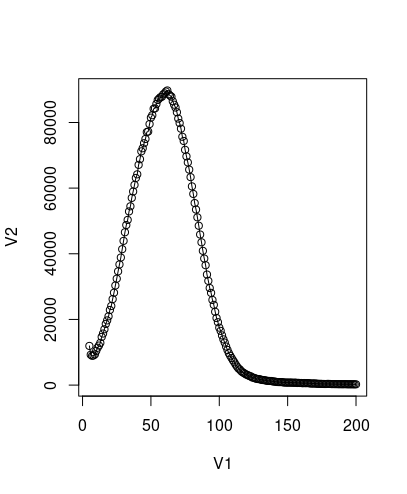
\includegraphics[scale=0.5 ]{peak1} 
	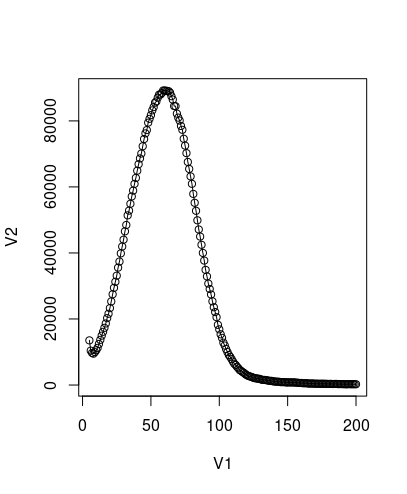
\includegraphics[scale=0.5 ]{peak2} \\
	
	\centering \caption{The k-mer distribution in the forward and reverse data among region between 8 and 200}
	\label{saw}
\end{figure}

%\begin{figure}[h]
%	\centering
%	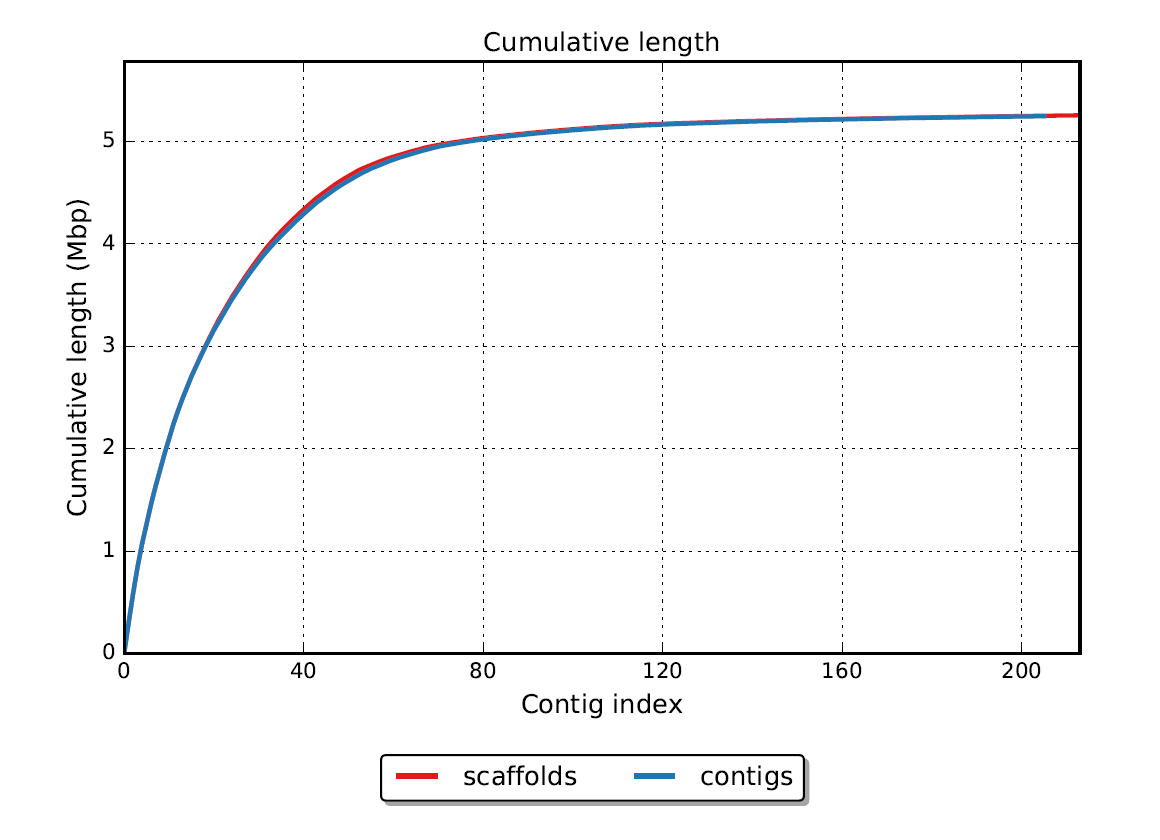
\includegraphics[scale=0.5 ]{images/consca.png} 
%	\centering \caption{Assessment of the quality of the paired processed data after using SPAdes}
%	\label{scacof}
%\end{figure}
The information related to the quality of the resulting assembly after SPAdes usage is available in lab journal.
Using Jellyfish we detemnied k-mer paek bin. For paired-end data the k-mer peak was 125. Depth of coverage was calculated according to formulas described in Methods. To calculate T(total bases number), the number of reads(5499436) was multiplied to average read length(90). These numbers were obtained from FastQC reports(see GitHub repository, as also R script to k-mer counting).As a result, estimated genome size is ~ 5.3 Gb and depth coverage is ~ 188.
After reads correction using SPAdes, k-mer profile hasn't changed. There is no significant improvement in k-mer distribution, except first bins. Genome size and depth coverage showed insignificant changes.
\subsection{ Checking assembly quality using QUAST}
	\begin{table} 
	\centering
	\begin{tabular}{|c|c|c|}
		\hline
		 & PE & PE+MP   \\
		\hline
		N50   & 105346  & 155269 \\
		\hline
		Number of contigs $\geq$ 50 bp & 205 & 169\\
		\hline
		Total number of contigs & 519 &  544 \\
		\hline
	\end{tabular}
	\caption{  Quality metrics of SPAdes assemblies. }
	\label{tab:2}
\end{table}
In this report, only basic metrics(such as N50,L50 and number of contigs with length more/equal than 500bp) will be reported. You can find the results in Table 2.
To sum up, addition of mate-pair libraries inproved N50 metric and contigs number, as expected. This fact could be easiy explained because addition of mate-pair sequencing libraries can negate problems in de novo genome assemblies. Mate pairs cover greater distances because of the increased insert size. As a result, they can cover genome regions that contain repeats. And  paired-end reads could fill the gaps between mate-pair reads. This approach (combinig mate-pair/paired-end reads) allows us to obtain better assemblies than just using one library type.
\subsection{Genome annotation and 16S rRNA study}
Next step was genome annotaion using Prokka. Results are:
-5064 CDS
-2923 genes
-80 tRNAs were found.
To find the closest reference genome, 16S rRNA prediction was performed. 16S rRNA is widely used for phylogenetic studies because 16S rRNA gene is highly conserved between different species of bacteria and archaea.
20 rRNA sequences were found in total, and 8 copies of 16S rRNA were found. Their length is 1536 bp for 7 copies and 406 bp for 1 copy. Using BLAST we successfully identified closest relative strain for our E.coli X strain. This is E.coli strain 55989($NC_011748.1$). BLAST reporting $100\%$ identity and cover. This newfound strain wiil be later used as a reference.
\subsection{ Genome-wide comparison using MSA} 
To find and see changes between X strain and 55989 strain, multiple sequence alignment using Mauve tool was performed. Using the fact that Shiga toxins can cause HUS, we searched results using Sequence Navigator. As a result, 2 genes (stxA and stxB) were found. These genes encoding A and B subunit of Shiga-like toxin which is repsonsible for 2011 HUS outbreak. To find how these genes were acquired, regions surrounding stx genes were investigated using Mauve GUI. Severel phage-related genes and also mobile element-related genes were found. We can assume that E.coli X contain not only pAA plasmind which has enteroaggregative genes, but also was infected by bacteriophage. We suggest that this phage was a deliverer and source of these toxins.
\subsection{Antimicrobial drug resistance analysis}
To analyse our refernce strain and X strain, ResFinder tool was used.
After analyzing both reference and target strains with ResFinder, it was found that the former is resistant to tetracycline due to production of tetB protein which is responsible for the drug efflux and acts as a metal-tetracycline/H+ antiporter in the cell. We can definitely say that X strain is almost a superbug because it has multiple resistance--t was reported to be resistant to cefepime, ampicillin, cefotaxime, sulfamethoxazole, trimethoprim and ceftazidime in addition to tetracycline. Most of its resistance was caused by beta-lactamase production. To track the source of this shocking fact Mauve tool was again used, as also the same approach(scanning regions nearby resistance genes). At least 2 enzymes were found: beta-lactamase CTX-M1 and beta-lactamase TEM. And these enzymes were flanked by mobile element-related sequences and/or phage genes responsible for phage replication. So, phage infection could be responsible not only for stxA/B genes, but also for AMR genes. In addition to that, in case of CTX-M1, there was a large insertion that was labeled as Incl1 plasmid transfer proteins. \# What a day, huh? Genome of X strain is a mish-mash but thus bacteria is a real danger

  
\section{Discussion}
X strain of E.coli is a claer example of horizontal gene transfer. First we found that Shiga-like toxins genes were surrounded by phage proteins. Second, in the case of beta-lactamase CTX-M-1, there is a large insertion containing genes from the Incl1 plasmid. As expected, both groups were absent in the reference genome. However, there is a strong possibility that the mechanisms of obtaining these genes differ. Let's talk about these mechanisms.

In the case of Shiga-like toxins, we could blame the phage integration mechanism. Phage life cycles dictate their role in bacterial and archaeal biology. Three life cycles of phages have been reported: lytic, lysogenic and chronic phages. In general, once a virulent phage (a phage that follows the lytic cycle) has attached to its host cell, the phage’s nucleic acid enters the cell and causes the bacterium to produce hundreds of phage copies. This results in the lysis of the cell and the newly formed phages are released into the surrounding environment. Temperate phages (phages that follow the lysogenic cycle) may follow one of two scenarios. The first scenario results in the lysis of the host cell and release of newly formed phages, similar to the lytic life cycle outlined above. In the second scenario, phage DNA may be integrated into the bacterial chromosome. The integrated DNA (prophage) is non-infectious and replicates as part of the bacterial chromosome. Incorporation of the phage DNA into the bacterial chromosome can be beneficial for the evolution of the bacteria as useful genes may be transferred to the bacteria. These prophage-mediated changes have been termed lysogenic conversion. In this state of symbiosis, both phage and the host cell experience an increased level of fitness. Under UV light or certain chemical treatments, the prophage is excised and causes the bacteria to produce phage particles. Figure 2 depicts the lytic and lysogenic lifecycle. The third life cycle is the chronic lifecycle which occurs in archaeal viruses and some filamentous and temperate phages. These viruses do not cause cell disruption or cell death, but instead the newly formed virions are continuously released from the cell. The infected host cells are capable of growing but at a much slower rate. You can read more here \cite{ncb}.

In case of antimicrobial resistance, the situation is a little more complicated. We can assume that E. coli X obtained the TEM beta-lactamase with the help of bacteriophages, as in the case of Shiga-like toxins. 
But the situation is different in the case of beta-lactamase CTX-M-1. Mauve exploration of neighbouring regions showed that the large insertion containing CTX-M-1 came from the Incl1 plasmid. Several studies show that this plasmid indeed contains such enzyme and can be transferred horizontally by conjugation process \cite{nature}. But also this insertion was also surrounded by phage proteins (e.g., phage minor tail protein, phage endopeptidase), according to the annotation. We can suggest with a strong confidencethat E. coli X obtained this gene via Incl1 plasmid since the insertion size is rather big and there are only a few phage genes around. Insertion size is too big to be carried by the phage, but from where these pheage genes occur? The exact way of transferring this gene to the strain of interest remains unknown. 
However, the mechanism of antimicrobial resistance in the case of beta-lactamases is clear. Beta-lactamases are enzymes that are responsible for the hydrolysis of the $\beta$-lactam ring of the antibiotic, making it ineffective. Most part of antibiotics that E. coli X is "immune" to compared to the reference strain (cefepime, cefotaxime, ampicillin and ceftazidime) belong to the class of  $\beta$-lactam antibiotics. But X strain also carries genes of sulfonamide (sul1, sul2) and trimethoprim (dfrA7) resistance which are capable of maintaining their function in presence of these antibiotics, thus making it superbug. HUS syndrome, multiple AMR--I'm concerned.

The simplest way to overcome such resistance is to use a combination of  $\beta$-lactam antibiotics with beta-lactamase inhibitors (e.g. clavulonic acid). You can check other methods in 1st report of our group in our GitHub repository.
Thank you for your attention!
 
%\newpage 
%\newpage 
\begin{thebibliography}{9}
 \bibitem{data}
 Datasets:  (forward and reverse) \\
SRR292678: \\
https://d28rh4a8wq0iu5.cloudfront.net/bioinfo/SRR292678sub\_S1\_L001\_R1\_001.fastq.gz \\ https://d28rh4a8wq0iu5.cloudfront.net/bioinfo/SRR292678sub\_S1\_L001\_R2\_001.fastq.gz \\
SRR292862: \\
https://d28rh4a8wq0iu5.cloudfront.net/bioinfo/SRR292862\_S2\_L001\_R1\_001.fastq.gz \\ https://d28rh4a8wq0iu5.cloudfront.net/bioinfo/SRR292862\_S2\_L001\_R2\_001.fastq.gz \\
SRR292770: \\
https://d28rh4a8wq0iu5.cloudfront.net/bioinfo/SRR292770\_S1\_L001\_R1\_001.fastq.gz \\
https://d28rh4a8wq0iu5.cloudfront.net/bioinfo/SRR292770\_S1\_L001\_R2\_001.fastq.gz

 \bibitem{fc}
 Fastqc : https://www.bioinformatics.babraham.ac.uk/projects/fastqc/
 
 
 \bibitem{jellyfish}
 Guillaume Marcais and Carl Kingsford, A fast, lock-free approach for efficient parallel counting of occurrences of k-mers. Bioinformatics (2011) 27(6): 764-770 (first published online January 7, 2011) doi:10.1093/bioinformatics/btr011
 
 
 \bibitem{spades}
SPAdes: http://cab.spbu.ru/software/spades/


\bibitem{quost}
QUAST: http://quast.bioinf.spbau.ru/

\bibitem{nature}
Knudsen, P.K., Gammelsrud, K.W., Alfsnes, K. et al. Transfer of a bla CTX-M-1-carrying plasmid between different Escherichia coli strains within the human gut explored by whole genome sequencing analyses. Sci Rep 8, 280 (2018). https://doi.org/10.1038/s41598-017-18659-2

\bibitem{prokka}
Seemann T.
Prokka: rapid prokaryotic genome annotation
Bioinformatics 2014 Jul 15;30(14):2068-9.


\bibitem{ncb}
Stone E, Campbell K, Grant I, McAuliffe O. Understanding and Exploiting Phage-Host Interactions. Viruses. 2019;11(6):567. Published 2019 Jun 18. doi:10.3390/v11060567

\end{thebibliography}




\end{document}
